\documentclass[../main.tex]{subfiles}
\graphicspath{{\subfix{../images/}}}
\begin{document}

\begin{figure}[h]
    \centering
    \begin{subfigure}[b]{0.1575\linewidth}
        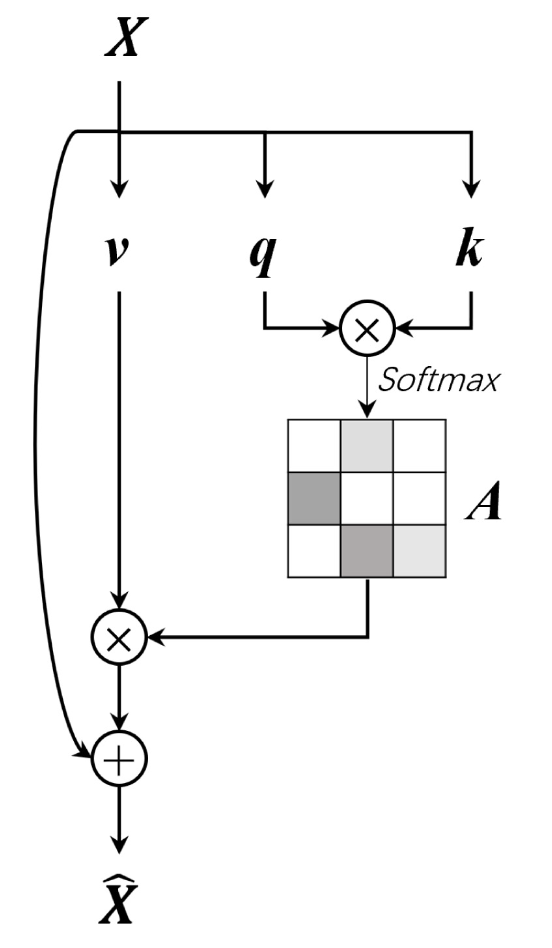
\includegraphics[width=\linewidth]{Siam_SR.png}
        \caption{Siam-SR}
    \end{subfigure}
    \hspace{0.1\textwidth}
    \begin{subfigure}[b]{0.3\linewidth}
        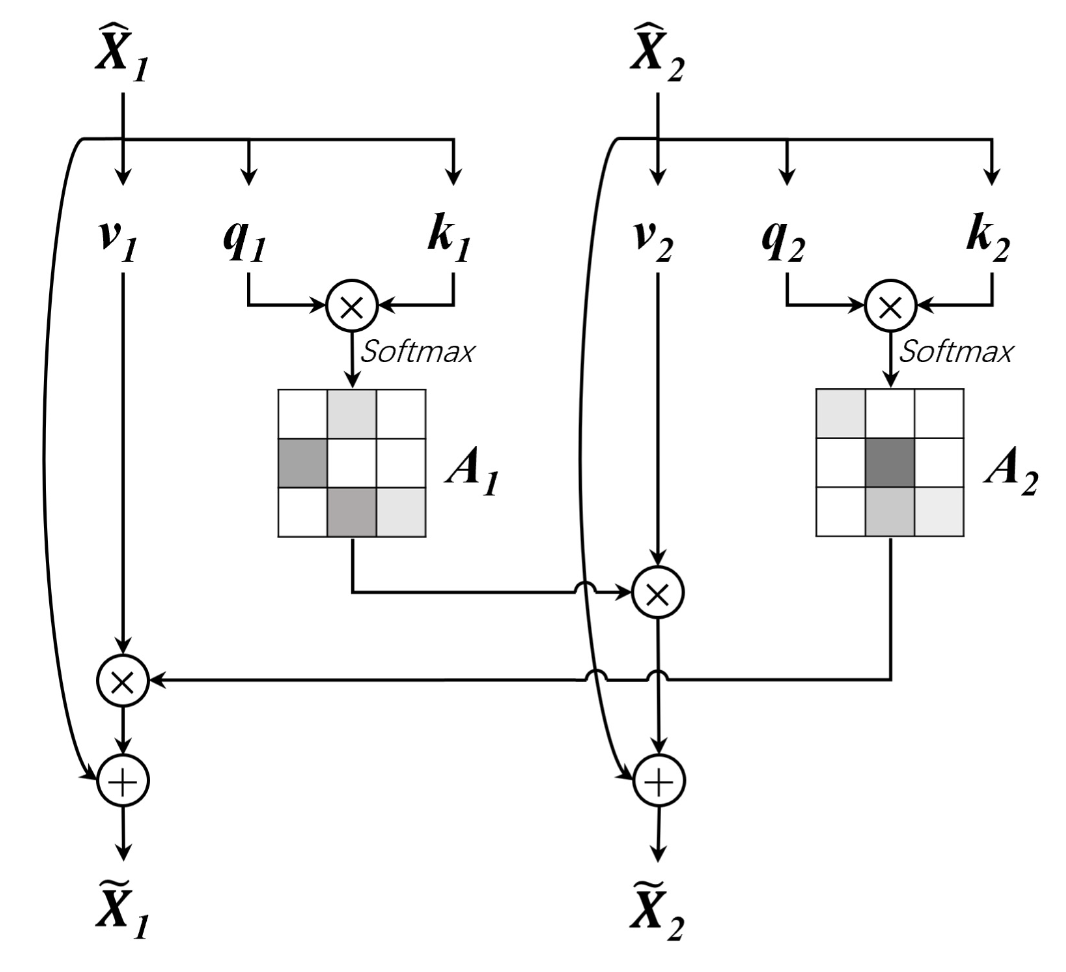
\includegraphics[width=\linewidth]{Cot_SR.png}
        \caption{Cot-SR}
    \end{subfigure}
    \caption{Structure of Siam-SR and Cot-SR blocks\cite{Ding_2022_Bi_SRNet}}
    \label{fig:attention_blocks}
\end{figure}

We noticed that the baseline model change network has two problems. First, it lacks the consideration of the semantic information in each temporal branch. Second, it lacks the consideration of the temporal correlations between two temporal branches. To address these issues, we added two feature attention blocks to the baseline model.

We use two blocks for feature attention; The Siamese semantic reasoning(Siam-SR) block and the Cross-temporal semantic reasoning(Cot-SR) block. Siam-SR block models the semantic information in each temporal branch. Cot-SR block models the temporal correlations between two temporal branches\cite{Ding_2022_Bi_SRNet}. Figure \ref{fig:attention_blocks} shows the structure of the two blocks.

Figure \ref{fig:baseline_with_attention} shows how we added Siam-SR and Cot-SR blocks to the baseline model. Siam-SR and Cot-SR blocks are memory intensive. To mitigate the memory issue, we added a max pooling layer before the Siam-SR block to reduce the dimension. We did not want to lose details from max pooling. Thus, we used the original features, as well as the features after attention, for the input to the change network. We achieved this by restoring the dimension of the features after attention with a bilinear interpolation layer, and concatenating these features with the original features.

\end{document}